\chapter{Adapting Latent Dirichlet Allocation to Overlapping Community Detection}
\doublespacing
\label{chap:lda}
\minitoc

\section{Introduction to the Latent Dirichlet Allocation Adaptation}
In Natural Language Processing (NLP), Latent Dirichlet Allocation (LDA) \cite{blei2003latent} is a classical document clustering method, a Bayesian network that models how documents in a corpus are topically related.
It is used to detect latent topics from documents by constructing a three-layer probabilistic graphical model: document-topic-word. In this three-layer model, documents and words can be observed from a dataset, while topics are a hidden layer which has to be estimated from the observed data.  
In StackOverflow, a user submits a question, then assigns 1$\sim$5 tags to indicate the key topics touched by this question. Other users who are interested in the question may provide answers to the question or comment on the question or others' answers. Therefore the main structuring graph in StackOverflow is the question-answer graph. As tags attached to a question  reflect its scope and domain, users answering a question can be considered as interested by this domain. As a result, a first approach to detect user communities is to consider that a user answering a question acquires the tags attached to this question and that gradually, each user acquires a list of tags associated with frequencies. If we treat the user as a document and tags acquired by the user as words in a document, then community detection can be considered as a clustering problem where users with similar topics of interest are grouped into the same cluster forming a community of interest.


\subsection{Problem Definition: mining topics and communities}

The problem of mining topics and communities in Q\&A platforms can be formalized as follows:

Let $U=\{u_1,u_2...u_n\}$ be the set of users, $Q=\{q_1,q_2...q_m\}$ the set of questions and $T=\{t_1,t_2...t_v\}$ the set of tags. We aim at:

\begin{enumerate}
 \item extracting topics distribution $Topic=\{topic_1,topic_2...topic_k\}$ from $T$, and for each $topic_k$, defining $topic_k=\{p_{k1},p_{k2}...p_{kv}\}$ where $p_{ki}$ denotes the probability of tag $t_i$ to be related to $topic_k$; an then
  \item detecting user's interests. For a user $u_i \in U$, we define $I_i=\{I_{i1},I_{i2}...I_{ik}\}$ where $I_{ik}$ denotes the probability of $u_i$ to be interested in $topic_k$.
\end{enumerate}

Similarly to \cite{Li:2010:CTM:1871437.1871673}, we applied the classic LDA method to construct a users-topics-tags model to detect latent topics of interest from the tags acquired by users and then cluster users into different topics. The output of the model consists of two probability distributions:
\begin{enumerate}
 \item a User-Topic distribution to describe to what extent a user is interested in the different topics.
 \item a Topic-Tag distribution to describe to what extent a topic is related the different tags.
\end{enumerate}



The formalization of this model is given by equation~\ref{eq:general}: 
\begin{equation}
P(t|u)=P(t|z)*P(z|u)
\label{eq:general}
\end{equation}
where $t$ denotes a tag, $z$ denotes a latent topic, $u$ denotes a user. The probability of a tag for a user is the result of multiplying the probability of this tag for a topic and the probability of this topic for the user.

Probabilistic graphical models (PGM) express the conditional dependence structure between random variables as a graph. 
The plate notation of the PGM of our model is presented in Figure \ref{fig:lda}. 
The variables appear as white disks if the variable is observed and blue disks if the variable is hidden (guessed), and blue disk written $\alpha$ and $\beta$ are hyper parameters of the model.
The dependencies among the variables are captured by the direction of the edges. 
The boxes represent replicated variables, which are users, topics (interests) and tags. 
%TODO Cath : In the figure the box Topic is not an inner box. I suppose the next sentence must be revised
%NOTE Zide the topic box (z) is an inner box.
%explained.
The Topic box represents different topic-tag distributions for each topic.
The User box represents different user-topic distributions for each user.
the Tag box represents one topic for each tag for each user.

The parameters of this model are explained in Table \ref{tab:parameters}.
$M$ and $V$ are given while $K$, $\alpha$ and $\beta$ can be chosen. $T$ is observed through the users' tag lists. Other variables are latent variables which have to be estimated.

\begin{figure}[htbp]\centering
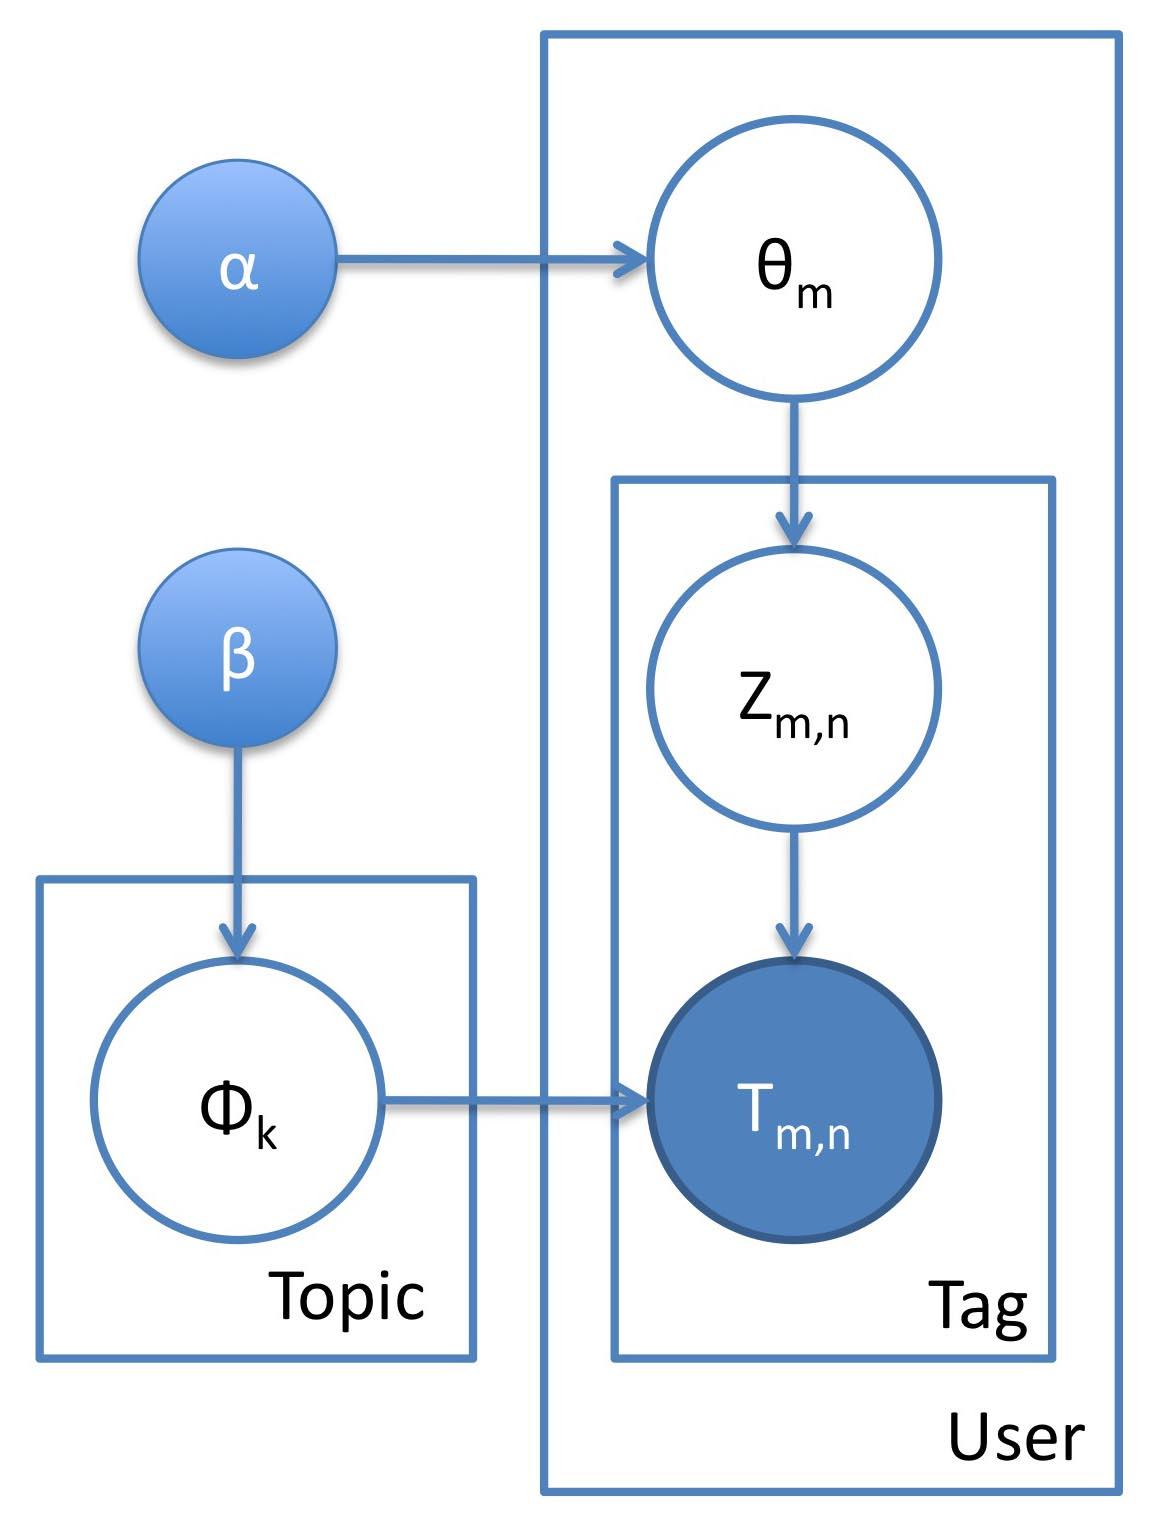
\includegraphics[ width=3.0in]{lda.jpg}  % "pdflatex"
\caption{User-Topic-Tag (LDA) Model}
\label{fig:lda}
\end{figure}

The intuition behind this model is that users choose their topics and that these chosen topics drive the generation of the tags.
The generative process can be summarized as follows:

\begin{algorithm}%[htp]
\begin{algorithmic}[1]
\label{algo:algoldagenerateprocess}
\State \textbf{Process of generating a user tag list} 

\For { \textit{topic k} \textbf{in} \textit{[1...K]} }
\State draw topic-tag distribution $\phi(k)$ $\sim$ Dir($\beta$)
\EndFor
\For { \textit{user m} \textbf{in} \textit{[1...M]} }
\State draw a user-topic distribution $\theta(m)$ $\sim$ Dir($\alpha$)
\EndFor
\For { \textit{tag} $T_{m,n}$ \textbf{in} \textit{ n \in [1...N_m], m \in [1...M]}}

\State draw topic $z_{m,n}$  $\sim$ Multi($\theta(m)$)
\State draw tag $t_{m,n}$ $\sim$ Multi($\phi(z_{m,n})$)

\EndFor
\end{algorithmic}
\end{algorithm}



%\noindent\rule[0.5ex]{\linewidth}{1pt}
%\textbf{Process of generating a user's tag list}\\
%\noindent \textbf{for} interest k \textbf{in} [1..K]:\\
%\indent draw topic tag distribution $\phi(k)$ $\sim$ %Dir($\beta$)\\
%\noindent \textbf{for} user $m \in [1,M]$:\\
%\indent draw a user-topic distribution $\theta(m)$ %$\sim$ Dir($\alpha$)\\  
%\indent \textbf{for} each tag $n \in$   user $m$'s tag %list, where $n~\in~[1,N_m]$, $m~\in~[1..M]$\\
%\indent \indent draw topic $z_{m,n}$  $\sim$ %Multi($\theta(m)$)\\
%\indent \indent draw tag $t_{m,n}$ $\sim$ %Multi($\phi(z_{m,n})$)\\ 
%\noindent\rule[0.5ex]{\linewidth}{1pt}

\begin{table}[htbp]
\caption{Model parameters}
\label{tab:parameters}
\centering
\begin{tabular}{|c|c|}
\hline
Parameter & Meaning \\
\hline
$M$ & the total number of users\\
\hline
$K$ & the total number of topics\\
\hline
$V$ & the total number of tags\\
\hline
$N_m$ & the total number of tags for user $m$\\
\hline
$\alpha$ & the parameter of the Dirichlet prior on the per-user topic distributions \\
\hline
$\beta$ & the parameter of the Dirichlet prior on the per-topic tag distributions  \\
\hline
$\theta_m$ & the topic distribution for user $m$ \\
\hline
$\phi_k$ & the tag distribution for topic $k$ \\
\hline
$z_{m,n}$ & the topic for the $n^{th}$ tag in $m$'s tag list \\
\hline
$t_{m,n}$ & the specified tag at the $n^{th}$ position in $m$'s tag list\\
\hline

\end{tabular}
\end{table}

We use the collapsed Gibbs Sampling method~\cite{griffiths2004finding} to sample the hidden variable $z$, then $\theta$ and $\phi$ can both be estimated.
The inference process is as follows.
We iteratively sample the topic indicator $z_{m,n}$ for each answer tag $t_{m,n}$ according to equation \ref{eq:ldasample}:

\begin{equation}
\begin{split}
p(z_i= z_{m,n} |u=u_m, t=t_{m,n}, Z, U, T_{\neg i}) &\\
\propto \frac{ C_{u_m,\neg i}^{z_{m,n}} + \alpha }{ \sum_{k=1}^K C_{u_m,\neg i}^k + K* \alpha} &\\
\cdot   \frac{ C_{z_{m,n},\neg i}^{t_{m,n}} + \beta }{ \sum_{t=1}^V C_{z_{m,n},\neg i}^t + V* \beta} &\\ 
\end{split}
\label{eq:ldasample}
\end{equation}

\noindent
where $\neg i$ enforces that all the counters used are calculated with tag $t_i$ excluded. $C_{u,\neg i}^k$ is the number of tags acquired by user $u$ assigned to topic $k$, $C_{k,\neg i}^{t}$ is the number of tags $t$ assigned to topic $k$.

Then with a Gibbs sampling, we can estimate $\theta$ and $\phi$ by equation \ref{eq:computetheta} and \ref{eq:computephi}:

\begin{equation}\scriptsize
\theta=\frac{ C_u^k + \alpha}{ \sum_{k=1}^K C_u^k+ K* \alpha}
\label{eq:computetheta} 
\end{equation}
\begin{equation}\scriptsize
\phi =\frac{ C_k^t + \beta}{ \sum_{t=1}^V C_k^t+ V* \beta}
\label{eq:computephi} 
\end{equation}

\noindent
where $C_u^k$ is the number of tags assigned to topic $k$ of user $u$ , $C_k^t$ is the number of tags $t$ assigned to topic $k$.


\section{First experiments: finding topics and communities with adapted LDA}

We ran the above described model on a dataset from the popular Q\&A site StackOverflow between 2008 and 2009, which is available online\footnote{\url{https://archive.org/details/stackexchange}}. Some basic statistics of the dataset are given in Table \ref{tab:stackoverflowdata}. We see that the total number of users is around 100K and among them, 47K users submitted at least one question, and 54K users answered at least one question. The total number of tags attached to questions is 24K, and 20\% of them are used more than 10 times. The frequency of tags follows a power law distribution. The total number of posts is 1.1M; among them there are 242K questions and 870K answers. Each question is attached with 1 to 5 tag as a tag list. Each user being represented by her tag lists. 

\begin{table}[htp]
\caption{Basic statistics of the stackoverflow dataset}
\label{tab:stackoverflowdata}
\centering
\begin{tabular}{|c|c|c|c|c|}
\hline
\textbf{item} & \textbf{description} \\
\hline
total number of users & 103K (47K questioners, 54K answerers)\\
\hline
total number of tags & 24K (20\% used more than 10 times)\\
\hline
total number of posts & 1.1M (242K questions, 870K answers) \\
\hline
\end{tabular}
\end{table}


We implemented the LDA algorithm in Python to create a user-topic-tag model as explained above.
A first result when running the algorithm is the probability for each tag to belong to each topic. 
Table \ref{tab:ldaresult1} shows eight examples of the detected topics of interest, each column showing one topic, and the ten rows giving the top 10 tags for each topic, sorted by descending weights. The weight of a tag is the probability of the tag to belong to the topic.  
This table shows that each topic has a clear and focused interest. For example, topic 1 has c-development related tags, topic 2 has java-development related tags, topic 3 has c\#-development related tags, topic 4 has html-development related tags, topic 5 has iphone-development related tags, topic 6 has database related tags, topic 7 has linux-development related tags, topic 8 has non-programming related tags. 
Moreover, weights reflect the relevance of tags to each topic. For example, topic 5 is concerned with iphone-development and its top 3 tags are 'iphone', 'objective-c' and 'cocoa' which are indeed very relevant.
\begin{sidewaystable}
\centering
%\begin{tabular}{|p{40pt}||p{40pt}||p{40pt}||p{40pt}|}
\begin{tabular}{|l|l|l|l|}
\hline
\textbf{\textcolor{blue}{topic 1}} &\textbf{\textcolor{blue}{topic 2}}  & \textbf{\textcolor{blue}{topic 3}}  & \textbf{\textcolor{blue}{topic 4}}  \\
\hline
%\multicolumn{4}{|c|}{c++(0.225), c(0.084), java(0.345), java(0.345), java(0.345), java(0.345), java(0.345), java(0.345), java(0.345), java(0.345)}\\
%\hline
 \textbf{c++}(0.225)& \textbf{java}(0.345)& \textbf{c\#}(0.225)& \textbf{php}(0.117) \\ 
\hline
 \textbf{c}(0.084)& \textbf{eclipse}(0.023)& \textbf{.net}(0.128)& \textbf{javascript}(0.115) \\ 
\hline
 \textbf{windows}(0.020)& \textbf{swing}(0.015)& \textbf{asp.net}(0.059)& \textbf{html}(0.059) \\ 
\hline
 \textbf{stl}(0.014)& best-practices (0.014)& \textbf{vb.net}(0.019)& \textbf{jquery}(0.056) \\ 
\hline
 algorithm(0.014)& multithreading (0.011)& \textbf{linq}(0.018)& \textbf{css}(0.042) \\ 
\hline
 c\#(0.013)& xml(0.010)& windows-forms (0.016)& mysql(0.029) \\ 
\hline
 \textbf{win32}(0.013)& \textbf{spring}(0.010)& \textbf{visual-studio} (0.015)& \textbf{ajax}(0.021) \\ 
\hline
 linux(0.011)& performance (0.009)& \textbf{asp.net-mvc} (0.015)& \textbf{web-development} (0.019) \\ 
\hline
 best-practices (0.011)& jsp(0.008)& wpf(0.012)& regex(0.018) \\ 
\hline
 multithreading (0.011)& generics(0.008)& best-practices (0.011)& \textbf{asp.net}(0.015) \\ 
\hline
\hline
\textbf{\textcolor{blue}{topic 5}} &\textbf{\textcolor{blue}{topic 6}}  & \textbf{\textcolor{blue}{topic 7}}  & \textbf{\textcolor{blue}{topic 8}}  \\
\hline
 \textbf{iphone}(0.137)& \textbf{sql}(0.181)& \textbf{python}(0.181)& subjective(0.143) \\ 
\hline
 \textbf{objective-c} (0.123)& \textbf{sql-server}(0.150)& \textbf{perl}(0.056)& \textbf{best-practices} (0.038) \\ 
\hline
 \textbf{cocoa}(0.080)& \textbf{database}(0.062)& \textbf{regex}(0.031)& \textbf{language-agnostic} (0.035) \\ 
\hline
 ms-access(0.062)& delphi(0.042)& \textbf{linux}(0.030)& programming (0.028) \\ 
\hline
 \textbf{cocoa-touch} (0.056)& \textbf{sql-server-2005} (0.042)& \textbf{ruby}(0.027)& \textbf{not-programming-related} (0.019) \\ 
\hline
 \textbf{iphone-sdk} (0.041)& \textbf{mysql}(0.039)& django(0.023)& \textbf{career-development} (0.018) \\ 
\hline
 vba(0.035)& \textbf{tsql}(0.037)& ruby-on-rails (0.021)& \textbf{learning}(0.017) \\ 
\hline
 excel(0.023)& \textbf{oracle}(0.028)& beginner(0.017)& polls(0.017) \\ 
\hline
 vb6(0.022)& \textbf{database-design} (0.025)& git(0.013)& programming-languages (0.015) \\ 
\hline
 xslt(0.021)& \textbf{stored-procedures} (0.017)& \textbf{bash}(0.013)& \textbf{design}(0.014) \\ 
\hline
\end{tabular}
\caption{Top 10 related tags for 8 detected topics of interest}
\label{tab:ldaresult1}
\end{sidewaystable}

The second result of the LDA algorithm is the probability for a user to belong to different topics of interest. 
Table \ref{tab:ldaresult2} shows six randomly chosen users and their top 10 tags. The first row contains user ids, the second row contains their detected topics of interest with their probability. The following ten rows show the top 10 tags for each user. We replaced topic ids with topic names which we have assigned to them according to their associated tags.
\begin{sidewaystable}%[htbp]
\centering
%\begin{tabular}{|p{60pt}|p{60pt}|p{60pt}|}
\begin{tabular}{|l|l|l|}
\hline
user\_21886&user\_14860&user\_15401\\
\hline
\textbf{\textcolor{blue}{html-development}} (0.284)  & \textbf{\textcolor{blue}{c-development}} (0.333) &\textbf{\textcolor{blue}{database-related}} (0.383)\\
 \textbf{\textcolor{brown}{c-development}} (0.275) &  \textbf{\textcolor{brown}{linux-development}} (0.196)& \textbf{\textcolor{brown}{non-programming-related}} (0.290)\\

\hline
python(93)&\textcolor{blue}{c}(152)&\textcolor{blue}{sql-server}(108)\\
%\hline
\textcolor{brown}{c++}(64)&\textcolor{blue}{c++}(148)&\textcolor{blue}{database}(64)\\
%\hline
\textcolor{blue}{javascript}(45)&java(89)&\textcolor{blue}{sql}(63)\\
%\hline
\textcolor{blue}{html}(34)&subjective(89)&\textcolor{brown}{subjective}(45)\\
%\hline
\textcolor{brown}{c\#}(33)&c\#(68)&python(43)\\
%\hline
\textcolor{blue}{css}(32)&sql(68)&\textcolor{blue}{sql-server-2005}(31)\\
%\hline
\textcolor{brown}{visual-studio}(29)&\textcolor{blue}{windows}(67)&\textcolor{brown}{best-practices}(27)\\
%\hline
\textcolor{brown}{windows}(27)&\textcolor{brown}{linux}(54)&.net(25)\\
%\hline
\textcolor{brown}{c}(27)&\textcolor{brown}{bash}(48)&c++(23)\\
%\hline
.net(24)&\textcolor{brown}{regex}(43)&c\#(22)\\
\hline
\hline
user\_78374&user\_53897&user\_23743\\
\hline
\textbf{\textcolor{blue}{non-programming-related}} (0.493)&\textbf{\textcolor{blue}{java-development}} (0.835)&\textbf{\textcolor{blue}{iphone-development}} (0.683)\\
\textbf{\textcolor{brown}{linux-development}} (0.316)&\textbf{\textcolor{brown}{non-programming-related}} (0.075)& \textbf{\textcolor{brown}{non-programming-related}} (0.155)\\

\hline
\textcolor{blue}{subjective}(35)&\textcolor{blue}{java}(366)&\textcolor{blue}{objective-c}(73)\\
%\hline
\textcolor{brown}{python}(32)&\textcolor{blue}{eclipse}(24)&\textcolor{blue}{cocoa}(71)\\
%\hline
\textcolor{blue}{best-practices}(16)&\textcolor{blue}{tomcat}(20)&\textcolor{blue}{iphone}(34)\\
%\hline
c(13)&\textcolor{brown}{subjective}(18)&\textcolor{blue}{cocoa-touch}(21)\\
%\hline
programming(13)&\textcolor{blue}{performance}(18)&\textcolor{blue}{mac}(19)\\
%\hline
c++(10)&\textcolor{brown}{best-practices}(16)&\textcolor{blue}{osx}(17)\\
%\hline
\textcolor{blue}{beginner}(8)&\textcolor{blue}{j2ee}(14)&\textcolor{blue}{iphone-sdk}(13)\\
%\hline
\textcolor{blue}{not-programming-related}(8)&\textcolor{blue}{jar}(13)&\textcolor{blue}{xcode}(10)\\
%\hline
\textcolor{blue}{language-agnostic}(6)&logging(10)&\textcolor{brown}{subjective}(8)\\
%\hline
\textcolor{blue}{coding-style}(5)&c\#(9)&c(8)\\
\hline
\end{tabular}
\caption{Detected topics of interest for 6 users}
\label{tab:ldaresult2}
\end{sidewaystable}

\section{Discussion: limitations and problems}
The above experiments verified that, by applying users-topics-tags models on Q\&A website, we are indeed able to detect overlapping communities, and that the detected topics are meaningful and could be used to explain the shared interest of each corresponding community as in our work, we directly use each topic to represent a community of interest.

However, we found that there are three limitations when applying LDA models to our task:

\begin{itemize}
\item The first one is a lack of efficiency: the complexity of the probabilistic model was prohibitive. \cite{chp7ldatimecomplexity} shows that the complexity of each iteration of the Gibbs sampling for LDA is linear with the number of topics and the number of documents, which is $O(kn)$, $k$ representing the number of topics, $n$ representing the number of posts. Besides, \cite{griffiths2004finding} proved that LDA model requires a few hundreds of iterations to obtain a stable topic distribution. Thus, it is necessary to improve the efficiency.

\item The second limitation is that the original LDA model does not enable to extract temporal and expertise information since the observed data in LDA model are limited to users and tags/words. However, there are actually more information that can be observed in the dataset, such as temporal information and vote information. For expertise modeling, we could not use votes directly because (a) the vote scores are sparse and noncontinuous, and (b) it is not reasonable to tell that a vote score $55$ is better than a vote score $50$ if the vote score are ranging from $0$ to $5000$. For temporal modeling, similar to \cite{wang2006topics} \cite{hu2014user}, we use time stamps directly. However, it is also important to extract temporal information in different point of view (year, month, day, hour).
Besides, contrary to \cite{blei2003latent} who applied LDA model on long documents such as news articles and assumed that each word has a latent topic, we assume  that each answer post has one topic: like in other social media with short contributions, e.g. Twitter, an answer post is normally short, each answer post is therefore suitable to be assigned with one single latent topic, and all the words in that post are considered to be generated by this topic. Some work \cite{chp7zhao2011comparing}\cite{chp7diao2012finding} on microblog also made this assumptions.

Therefore, we aim to extend the original LDA model to extract temporal and expertise information, which will be used to solve question routing task, etc. 



\item The third limitation is that the detected probability distributions cannot be compared with each other.  Let us explain this in detail. A three-layer LDA model (user-topic-word) generates two kinds of distributions, a user-topic distribution and a topic-word distribution, which describe to what extent a user is interested in different topics and to what extent a keyword or a tag is related to different topics. 
However, as shown in figure~\ref{fig:usertopic}, the same user-topic distribution could be generated by different training data (assume that the hidden variable topic is generated by Gibbs sampling~\cite{griffiths2004finding}), which means that user-topic distributions are incomparable among users. For the upper distribution of figure~\ref{fig:usertopic}, \emph{Alice} is more active in topic \emph{music}, but for the lower one, \emph{Bob} is more active. 


\end{itemize}

\begin{figure}
\centering
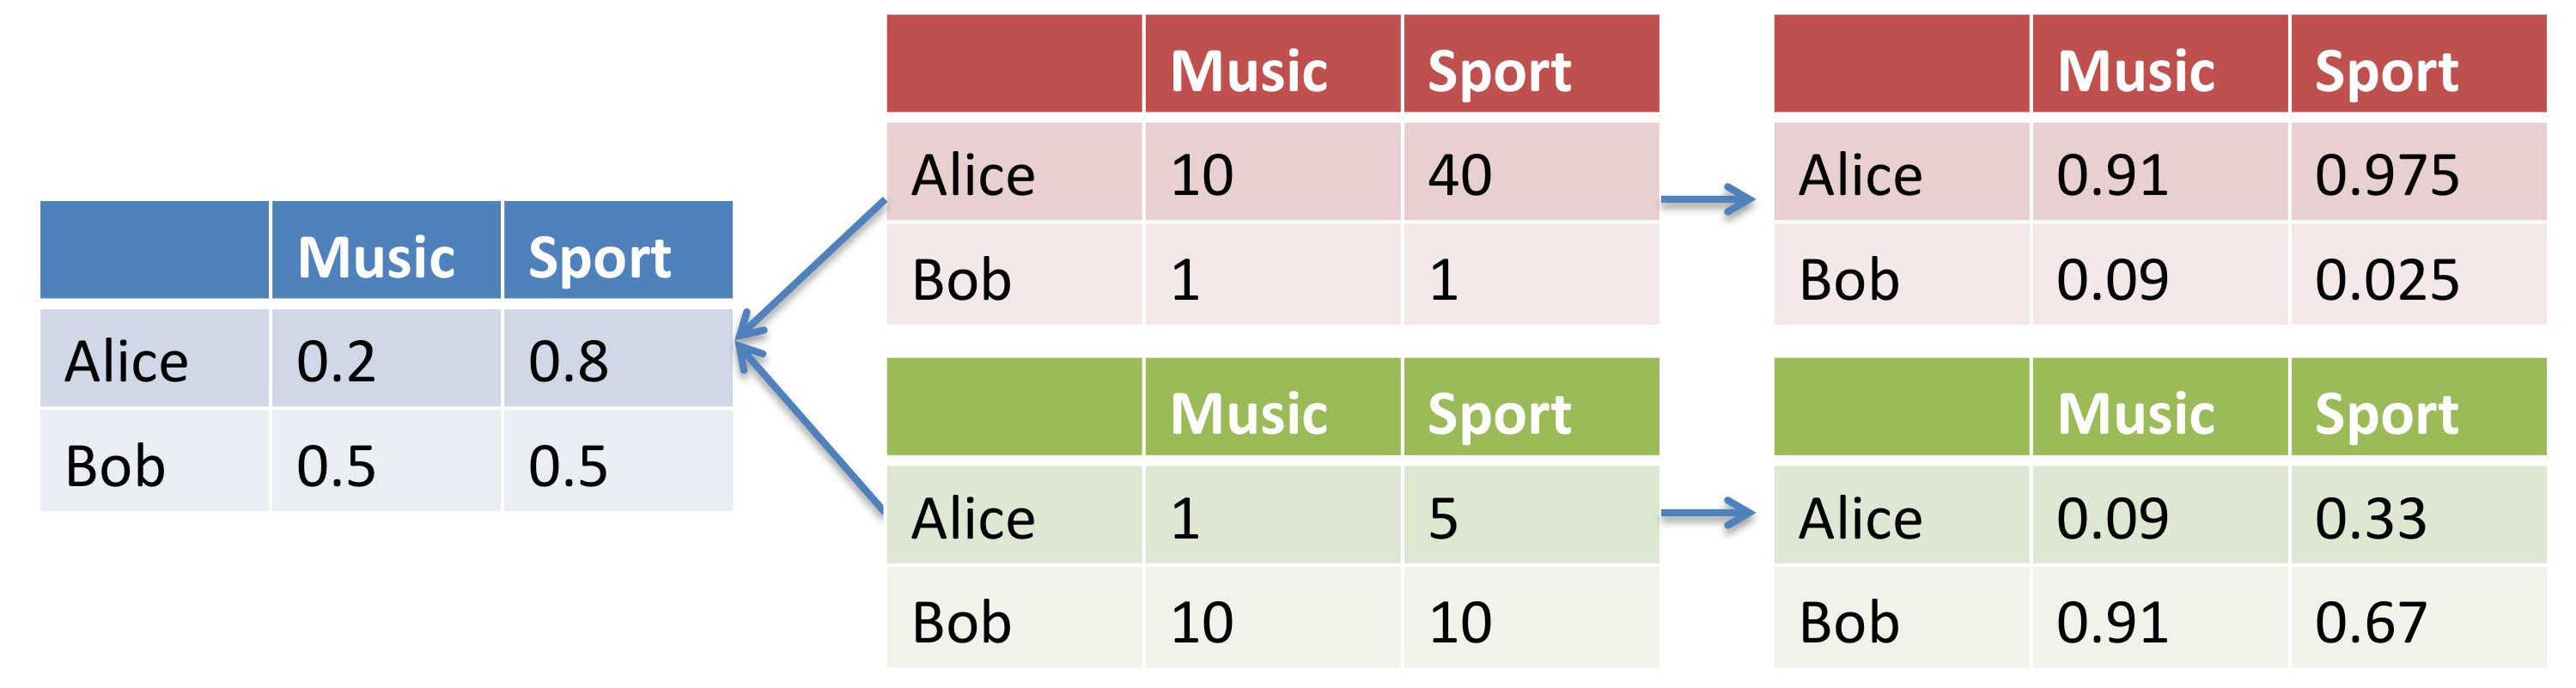
\includegraphics[ width=5.1in]{usertopic.jpg}  
%\caption{Different ways to estimate probabilities with Gibbs sampling results}
\caption{Different ways to estimate probabilities with topic assignment counts. Tthe upper table: per-user topic distribution; the bottom table: per-topic user distribution}
%\caption{Two examples of topic assignment counts normalization per user and per topic.
\label{fig:usertopic} 
\end{figure}


Therefore, in the rest of this thesis we show how we extended our preliminary work in two directions:

\begin{enumerate}
 \item First, we developed a more simple method to detect topics and overlapping communities to solve the efficiency problem: the TTD method is presented in Chapter \ref{chap:ttd}.
  \item Second, we propose a more complex model to extract more information from user generated content to answer the two other limitations: we propose the TTEA method to extract more information and a post-process method to solve the incomparable problem. They all described in Chapter \ref{chap:ttea}
\end{enumerate}
 
